\documentclass[letterpaper,12pt]{article}

\usepackage{float}
\usepackage{graphicx}
\usepackage{hyperref}
\usepackage{subcaption}

\title{Intro to Intelligent Security Systems: Project 1}
\author{Alvin Lin, Nathan Farrell, Peter Doyle}

\begin{document}

\maketitle

\section*{Executive Summary}
For project 1, we implemented structures for misuse and anomaly based IDS
systems. Through the combination of decision trees and using baseline metrics
to threshold anomalous traffic, our misuse and anomaly based IDS achieved
accuracy levels of 95\% and 74\%, respectively.

\section*{Specification}
For this project, we intend to design a technique to distinguish normal
connections from attacks in the data provided by the 1999 KDD Cup. The
techniques described below can be abstracted and applied to an IDPS but the
report will mostly focus on their application to the provided data. \par
Our anomaly based IDS will use the training data to calculate a standard for
normal traffic. Determining whether or not a network connection is anomalous
will involve determining its deviation from our calculated normal standard. In
contrast, our misuse based IDS will use a decision tree to evaluate the
attributes provided in the data to determine whether or not a connection is
anomalous. The decision tree will be built by inspection of the data. \par
To evaluate our system, we will be measuring its accuracy rate and
misclassification rate. Given the nature of an IDS system, we will attempt to
maximize the true positive rate and minimize the false negative rate.


\section*{Methods and Techniques}

\subsubsection*{Data Preparation}
In order to use the data from the 1999 KDD Cup, we had to preprocess it and
vectorize it for efficient handling. Preprocessing mostly involved parsing the
data from the file and correctly interpreting what the elements in each row
represented. Most of the data was already of interval type since they measured
absolute statistics about the connection with the exception of some nominal
metrics like flag, service type, and connection type. For these nominal values,
we assigned them each a unique integer identifier to make them easier to handle
in a \texttt{numpy} array. We split the labeled data from the KDD Cup into two
sets, one for training and the other for testing. \par

\subsubsection*{Misuse IDS}
The misuse IDS was created using a decision tree that was based off the manual
inspection of the 1999 KDD Cup data mentioned above. The tree itself has at most
four layers that the data coming in can branch down. The first layer of which is
the protocol of the data coming in (udp, icmp, or tcp). The second layer
branches on the service that the packet was sent through. Across the KDD Cup
data there were 65 services that the misuse IDS can successfully detect
anomalous data on. The third layer within the decision tree split the
information on the flag of the packet. The fourth layer used spcific attributes
to determine the type of anomalous behavior the packet is or whether it is
normal traffic. Each packet is input into the tree until it reaches the end and
is classified. The inspection of the data done beforehand led to an accurate
classification ratio. \par

\subsubsection*{Anomaly IDS}
The anomaly IDS used the training data to establish a baseline metric for
normal network connections. To do this, we isolated all the network connections
considered normal usage in the training data set and pruned out any outliers.
We took the median value of all the connections considered normal and used it
as the baseline for normalcy. To determine if a connection was considered
anomalous, we chose to use Minkowski distance as a measure of a connection's
distance from normalcy.
\[ D_p(X,Y) = \left(\sum_{i=1}^{n}|x_i-y_i|^p\right)^{\frac{1}{p}} \]
For this vector space with \( n = 40 \), we used a variant of Manhattan
distance by choosing \( p = 1 \). If the Minkowski distance was above a certain
threshold, we flagged the connection as anomalous. To determine an optimal
threshold, we used a tested a series of thresholds and generated a
receiver-operating characteric curve, selecting the one that would result in
the lowest misclassification ratio. \par
We calculated the misclassification rate na\"{i}vely by weighting both the
false positive rate and false negative rate equally using the following cost
function.
\[ Cost = (1\times FP) + (1\times FN) \]
For an IDS system, it would probably be recommended to reduce the false
negative rate, so weighting the false negatives higher when choosing a
threshold would also be a good choice.

\section*{Implementation}
This project was implemented in Python 3. We made use of the
\href{http://www.numpy.org/}{\texttt{numpy}}
library for fast vector operations and data manipulation. This allowed for
very easy data manipulation due to the syntactic sugar provided by Python and
the powerful indexing operations provided by \texttt{numpy}. We did not have to
compromise much on speed due to the optimized nature of \texttt{numpy} arrays.
In addition, we used the \href{https://matplotlib.org/}{\texttt{matplotlib}}
library to generate graphs and data visualizations. This helped us determine
attributes to split on when building the decision tree and visualized the
receiver-operating characteristic curve to pick a threshold for the anomaly
IDS. Both the preprocessing library, anomaly IDS, and misuse IDS frameworks were
written from scratch using only the libraries above.

\section*{Tests}
We used the labeled data from the 1999 KDD Cup to perform testing on both IDS
systems.

To determine the best threshold to use for the anomaly based IDP, we tested a
variety of thresholds against our training data.
\begin{figure}[H]
  \centering
  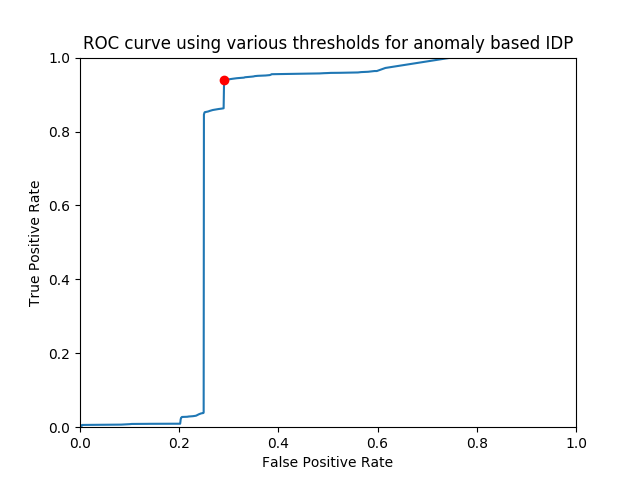
\includegraphics[width=12cm]{anomaly_roc.png}
  \caption{ROC curve for the anomaly IDP when testing thresholds.}
\end{figure}
We generated a receiver-operating characteristic curve for the anomaly IDP to
determine the optimal threshold. A threshold of 2230 in our scale space (marked
in red) resulted in the lowest misclassification rate for the anomaly based
IDP, but depending on the needs, a higher or lower threshold could be chosen. On
the training dataset, this threshold resulted in a 94\% true positive rate and
a 29\% false positive rate.

For the misuse IDS, to caliberate the decision tree to accurately classify the
data coming in, we manually inspected each different combination of protocol,
service, and flag in order to pick out the specific attributes that belonged
to certain types of anomalous or normal traffic. Each combination was tested
one by one until the decision tree had an accurate representation of the
different protocols, services, and flags that the IDS would experience. Once
the tree represented all of these different combinations, the IDS was able to
achieve the accuracy levels that are described below.
\section*{Results}
When the anomaly IDS was run on the testing dataset, we obtained the following
data:
\begin{center}
  \begin{tabular}{c|c|c}
    \( n = 211029 \) & Predicted Anomalous & Predicted Normal \\
    \hline
    Actually Anomalous & 124784 & 44788 \\
    \hline
    Actually Normal & 10948 & 30509
  \end{tabular}
\end{center}
Given that the original dataset had 169572 anomalous records and 41457 normal
records of network connections, this yielded us the following information:
\begin{itemize}
  \item Accuracy \( \frac{TP+TN}{total} \): 73.6\%
  \item Misclassification Rate \( \frac{FN+FP}{total} \): 26.4\%
  \item True Positive Rate \( \frac{TP}{TP+FN} \): 73.5\%
  \item False Positive Rate \( \frac{FP}{FP+TN} \): 26.4\%
  \item Precision \( \frac{TP}{TP+FP} \): 91.9\%
\end{itemize}
This is interesting because a completely na\"{i}ve model that simply flags
every connection as anomalous would have had an 80.3\% accuracy rate with a
100\% false positive rate. Minimizing the misclassification ratio reduced our
accuracy on the testing dataset to 73.6\% and our false positive rate to 26.4\%.

After running the validation data on the misuse IDS, there were 168700 true positives,
35468 true negatives, 5989 false positives, and 872 false negatives. leading to the
total accuracy of the program to be calculated at 96.7\%, the true positive rate being
79.9\% and the false positive rate being 2.8\%. All of which is run in 0.85s.

\section*{Development Process}
Due to Peter Doyle joining late, Alvin Lin was in charge of developing the
anomaly IDS and documenting that half of the documentation while Nathan Farrell
completed the misuse IDS and documented that half of the documentation. Nathan
spent around 6-8 hours on completing the misuse IDS and documentation. Alvin
spent 6-7 on the anomaly IDS and documentation. We are confident as a group
that Peter will make up for the lack of work done in future deliverables.

\end{document}
